\documentclass[12pt,titlepage]{article}


\usepackage{nomencl}
\usepackage[american]{babel}
\usepackage[utf8]{inputenc}
\usepackage[T1]{fontenc}
\usepackage{lmodern}
\usepackage{amsmath,amsfonts,amssymb}
\usepackage{graphicx}
\usepackage{geometry}
\geometry{a4paper}
\usepackage[parfill]{parskip}
\usepackage{graphicx}
\usepackage{amssymb}
\usepackage{epstopdf}
\usepackage{color}
\usepackage[tt]{titlepic}
\usepackage{fancyhdr}
\usepackage{enumerate}
\usepackage{lastpage}
\usepackage{bm}

\usepackage{listings}
\definecolor{codegreen}{rgb}{0,0.6,0}
\definecolor{codegray}{rgb}{0.5,0.5,0.5}
\definecolor{codepurple}{rgb}{0.58,0,0.82}
\definecolor{backcolour}{rgb}{0.95,0.95,0.92}
 
\lstdefinestyle{mystyle}{
    backgroundcolor=\color{backcolour},   
    commentstyle=\color{codegreen},
    keywordstyle=\color{magenta},
    numberstyle=\tiny\color{codegray},
    stringstyle=\color{codepurple},
    basicstyle=\footnotesize,
    breakatwhitespace=false,         
    breaklines=true,                 
    captionpos=b,                    
    keepspaces=true,                 
    numbers=left,                    
    numbersep=5pt,                  
    showspaces=false,                
    showstringspaces=false,
    showtabs=false,                  
    tabsize=2
}
 
\lstset{style=mystyle}

\usepackage[section]{placeins}
\usepackage{amsfonts}
\usepackage{amsmath}
\usepackage{float}
\usepackage{setspace}
\usepackage[justification=centering]{caption}
\usepackage{sidecap}
\usepackage{subcaption}
\usepackage{multirow}
\usepackage[squaren, Gray, cdot]{SIunits}
\graphicspath{{image/}} %chemin par défaut pour aller chercher les images 
\usepackage{url}
\usepackage[utf8]{inputenc}
% FOR DEFINITIONS (https://www.sharelatex.com/learn/Theorems_and_proofs)
\usepackage{amsthm}

\newtheorem{definition}{Definition}[section]
\newtheorem*{definition*}{Definition}
\newtheorem{prop}{Proposition}
\newtheorem*{prop*}{Proposition}
\theoremstyle{remark}
\newtheorem*{remark}{Remark}
\newtheorem*{corollary}{Corollary}
\newtheorem{theorem}{Theorem}[section]
\newtheorem{lemma}[theorem]{Lemma}
\newtheorem*{example}{Example}

% Custom Defines
\usepackage[comma,numbers,sort&compress]{natbib}
\bibliographystyle{plainnat}
\usepackage[pdfstartview=FitH,
            breaklinks=true,
            bookmarksopen=true,
            bookmarksnumbered=true,
            colorlinks=true,
            linkcolor=black,
            citecolor=black
            ]{hyperref}
\newcommand{\rmd}{\textrm{d}}
\newcommand{\bi}[1]{{\ensuremath{\boldsymbol{#1}}}}
\definecolor{gray}{rgb}{0.5,0.5,0.5}

\topmargin=-0.45in      %
%\evensidemargin=0in     %
\oddsidemargin=-0.1in      %
\textwidth=6.8in        %
\textheight=9.2in       %
%\headsep=0.25in         %
\headheight=30.9pt

\begin{document}

% ========== TITLE PAGE ===================================================

\begin{titlepage}
\newcommand{\HRule}{\rule{\linewidth}{1mm}} % Defines a new command for the horizontal lines, change thickness here

\center % Center everything on the page

\includegraphics[width=8cm]{Figs/Cover/polimi.png}\\[1.5cm]

\includegraphics[width=8cm]{Figs/Cover/EPFL.jpg}\\[1.5cm]
%	HEADING SECTIONS
\textsc{\LARGE Master Thesis in Computational Science and Engineering}\\[1.cm]

%	TITLE SECTION
\HRule \\[0.4cm]
{ \huge \bfseries About the convergence of the Graph Laplacian}\\[0.4cm] 
\HRule \\[1.5cm]     

%	AUTHOR SECTION
\begin{minipage}{0.4\textwidth}
\begin{flushleft} \large
\emph{}\\
Martino \textsc{Milani}\\
\end{flushleft}
\end{minipage}
~
%	DATE SECTION
{\large \today }\\[2cm] % Date, change the \today to a set date if you want to be precise
\vfill % Fill the rest of the page with whitespace
\end{titlepage}
%\onehalfspacing

% ========== HEADER =======================================================
\pagestyle{headings} \pagenumbering{arabic} \setcounter{page}{1}
\addtolength{\headheight}{\baselineskip}
\lhead{\textbf{Martino Milani}}
\chead{Master Thesis}
\renewcommand{\headrulewidth}{0.4pt}


\begin{abstract}
Problem definition: find a convergence result for the Graph Laplacian on a graph approximating a sphere (WHICH GRAPH? Because for a full graph with $W(i,j)=e^{||x_i-x_j||^2}$ we already have it) to the Laplace-Beltrami operator on the sphere, given a deterministic sampling (HealPix).


\end{abstract}
\pagebreak

\tableofcontents
\pagebreak

%\listoffigures
%\listoftables
%\pagebreak


%*******************************************************************************
%***********************************    Background   *****************************
%*******************************************************************************
%!TEX root = 0.main.tex

\setcounter{page}{1}



%********************************** %First Section  **************************************
\section {Introduction and general background} 

\subsection{Introduction}

Neural Networks (NNs) are popular algorithms for regression and classification tasks. Taking as example an image classification problem, a neural network perform multiple combinations of linear and non-linear transformations of each image $I$ to assign it a label $C_I$ chosen in the set of all the possible labels $\mathcal C$. The first \textit{layer} of the neural network transforms the input image $I$ in a vector - called \textit{feature map} - $\mathbf f_1$ through a function $\phi_1$.  The output feature map of the first layer is used as input of the second layer that transforms it through a function $\phi_2$, and so on, until the original image $I$ is mapped into a label $C_I$ by the last, $n$-th layer of the neural network:
$$C_I = \phi_n \circ \phi_{n-1}\circ ... \phi_2\circ\phi_1 (I)$$
 With a large \textit{training set} of pre labeled images at its disposal, a NN is capable of learning the optimal transformations $\phi_i$ that let it map each input image to its correct label. Since the functions $\phi_i$ have many degrees of freedom - even millions - a neural network is able to learn very complex transformations. In the work of Cs\'aji \cite{NN}, NNs have been proved to be universal function approximators, meaning that with a sufficient number of parameters NNs are able to approximate any continuous function on a compact domain. This makes NNs the optimal tool for complex tasks such as image classification, image segmentation, speech recognition and natural language processing.
 
Convolutional Neural Networks (CNNs) are a subset of NNs whose layer structure has been specifically designed for image recognition and segmentation. For this purpose, they don't have all the degrees of freedom of a \textit{fully connected} neural network: each layer is constrained to learn only those transformations of the input that are \textit{equivariant} to translations of the input. This means that a translation of the input image will not result in a change of class. The layers $\phi_i$ of a CNN are \textit{convolutions} with some kernels $k_i$, that were learned during the training phase. Thanks to their design, training of CNNs is faster - thanks to the smaller number of parameters to be learned compared to a fully connected NN -, easier - since there's no need of artificially \textit{augmenting} the dataset with translated copies of the same image -, and leads to very accurate results \cite{SCNN}, \cite{Esteves}.

Spherical convolutional neural networks (SCNNs) are CNNs that have been designed to deal with spherical data, whose layer design makes them equivariant to \textit{rotations} of the input.  Examples of tasks where data is naturally represented on a sphere are (i) climate science, where data is sampled on the surface of the Earth, (ii) cosmology, where observations are naturally projected on a sphere centered around the observer (see Figure \ref{fig:cosmicradiation}), and (iii) virtual reality, where the images are represented on a sphere centered around the player. Being able to come up with rotation equivariant architectures brings with it all the advantages that traditional CNNs have brought for traditional (euclidean) image classification tasks: training is faster, easier and results are very accurate. Each layer of a SCNN performs a \textit{spherical convolution} of the input feature map with a kernel $k_i$ learned during the training phase. One of the main issues with traditional SCNNs is the computational complexity of computing at each layer the Spherical Harmonic Transform of the data to perform the convolution. To overcome this issue, Perraudin et al. \cite{DeepSphere} proposed a Graph Convolutional Neural Network (GCNN) that is almost equivariant to rotations, replacing the SHT with a more efficient Graph Convolution.
\begin{figure}
	\centering
	\caption{\label{fig:cosmicradiation} Cosmic microwave background map, the oldest electromagnetic radiation in the universe. Source: Wikipedia}
	\includegraphics[width=0.4\textwidth]{figs/literaturereview/WMAP.png}
\end{figure}

This work is organized as follows: in Chapter 1 we start by presenting fundamental concepts of spectral theory on the sphere and we present classical ways of building rotation equivariant neural networks through the use of the classical SHT.  We present then some basics of Spectral Graph Theory that lay the foundations of Graph Convolutional Neural Networks.  In Chapter 2 we present the general framework of how to discretize the Laplace-Beltrami operator on a general manifold, concluding with the special case of the Heat Kernel Graph Laplacian (HKGL) approximation, together with some convergence results. We continue in Chapter 3 by introducing DeepSphere \cite{DeepSphere}, a Graph Spherical Convolutional Neural Network (GCNN) that uses a graph Laplacian matrix $\mathbf L$ similar to the HKGL to perform graph convolutions that are almost equivariant to rotations. We study the spectral properties and the equivariance error of DeepSphere and we show a way to build a graph $G'$ such that the corresponding graph Laplacian matrix $\mathbf L'$ shows better spectral and equivariance properties. In Chapter 4 we show better graph constructions than the HKGL on non uniform sampling measures. To conclude, we show a different approach to perform rotation invariant convolutions that uses the Finite Element Method (FEM) approximation of the Laplace-Beltrami operator on the the sphere. Chapter 5 concludes this work by presenting some experimental results obtained by Gusset et al. \cite{Gusset} that implemented the graph $G'$ on a GCNN and compared its performances to DeepSphere on a well known dataset \cite{SHREC17} showing that the new graph $G'$ performs better in real applications. We finish by comparing the FEM and the graph approach, discussing the general problem of how to incorporate geometrical informations about the sphere in the graph.

\subsection{Fourier Transforms and Convolutions on the 2-Sphere}\label{sec:Fourier on the Sphere}
The goal of this section is to present to the reader some fundamental results of spectral theory on the sphere that we will need in this work. We present a brief review of Banach and Hilbert spaces, spherical harmonics, Fourier transform and convolution on $\mathbb S^2$. We refer to Sections 2 and 3 of the work of Driscoll and Healy \cite{Driscoll:1994:CFT:184069.184073} for a more detailed and effective review of spectral theory on the Sphere.

\paragraph{Banach and Hilbert spaces.}
A \textit{norm} $\norm\cdot:\ X\to\mathbb R$ on a vector space $X$ is a subadditive, positive definite function such that $\norm{x+y}\leq\norm x +\norm y,\ \forall x,y\in X$ (triangle inequality). A \textit{Cauchy sequence} $(x_n)\subset X$ is a sequence such that $\forall \epsilon>0\  \exists M>0: $ $\forall i,j>M$ $ \norm{x_i-x_j}<\epsilon$. A \textit{Banach space} $(X, \norm{\cdot})$ is a normed vector space on the scalar field $F$ that is \textit{complete}, meaning that $X$ is "big enough" such that for every Cauchy sequence $(x_n)\subset X$ there exist a $x\in X$ such that $x$ is the limit of $(x_n)$ in $X$ i.e. $\norm{x_n-x}\rightarrow 0$. A \textit{basis} of $(X, \norm\cdot)$ is a minimal set of linearly independent vectors $\mathcal B \subset X$ such that every element of $X$ can be written as linear combination of the elements of $\mathcal B$. A scalar product is a function $\langle\cdot,\cdot\rangle: X\times X \rightarrow \mathbb F$ that is linear in the first argument, positive definite and conjugate symmetric. Through a scalar product we can define the notion of angle $\theta$ between two elements $x, y \in X$ through the following formula: 
$$
\cos \theta = \frac{\langle x, y\rangle}{\norm x \norm y}
$$ 
In particular we can define the notion of orthogonality: two elements  $x, y \in X$ are orthogonal if and only if $\langle x, y\rangle=0$. We are interested in those particular Banach spaces where we can define a notion of orthogonality between vectors. A Banach space $(X, \norm \cdot )$ is a \textit{Hilbert space} when the norm $ \norm \cdot $ can be induced by a \textit{scalar product}: $\norm \cdot = \sqrt{\langle\cdot,\cdot\rangle}$. We can now define an \textit{orthonormal} basis of $X$: a basis $\mathcal B \subset X$ such that $\forall x, y \in \mathcal B, \norm x = \norm y = 1 \text{and } \langle x, y\rangle = 0$. Given an orthonormal basis $\mathcal B = \{b_i\}_{i\in I}$ we can write each vector in its \textit{Fourier series} 
\begin{equation}\label{eq:abstract fourier}
x = \sum_{i\in I} \langle x, b_i\rangle b_i
\end{equation}
If the set $I$ is countable the Hilbert space $(X, \norm\cdot)$ is called \textit{separable}. Having a countable orthonormal basis, and thus the possibility of representing each vector through its Fourier series enormously simplifies many problems.
\paragraph{Spherical Harmonics.}
 Given the usual parametrization $x = x(\theta, \phi), \theta\in[0,\pi], \phi\in[0,2\pi]$ of the sphere
\begin{align*}
\mathbb{S}^{2}&=\left\{\omega=\left(\omega_{1}, \omega_{2}, \omega_{3}\right) \in \mathbb{R}^{3} :\|x\|_{\mathbb{R}^{3}}=\left(\omega_{1}^{2}+\omega_{2}^{2}+\omega_{3}^{2}\right)^{1 / 2}=1\right\}\\
\omega_{1}&=\cos (\phi) \sin (\theta), \quad \omega_{2}=\sin (\phi) \sin (\theta), \quad \omega_{3}=\cos (\theta)
\end{align*}
the Hilbert space $L^2(\mathbb S^2)$ is defined as the space of square-integrable functions endowed with the scalar product $\langle f,g\rangle=\int_{\mathbb S^2}f(\omega)\overline g(\omega)d\omega$ where the measure $d\omega$ is the rotation-invariant measure such that
\begin{align}
\int_{\omega \in \mathbb S^{2}} f(\omega) d \omega&=\int_{\phi=0}^{2 \pi} \int_{\theta=0}^{\pi} f(\omega(\theta, \phi)) \sin \theta d \theta d \phi\\
\int_{\omega \in \mathbb S^{2}} f(g \omega) d \omega&=\int_{\omega \in \mathbb S^{2}} f(\omega) d \omega, \quad g \in S O(3)
\end{align}

For each rotation $g\in SO(3)$ we define a corresponding rotation operator $\Lambda(g)$ by
\begin{equation}\label{eq:rotation operator}
	\Lambda(g) f(\omega)=f\left(g^{-1} \omega\right)
\end{equation}
A space is invariant under the rotations $g$ in $SO(3)$ if all operators $\Lambda(g)$ take each function of the space back into the space. As very well written by Driscoll et al \cite{Driscoll:1994:CFT:184069.184073}:

\vspace{0.2cm}
\textit{Fourier analysis on the sphere amounts to the decomposition of the space of square integrable functions on \(\mathbb S^{2}\) in minimal subspaces $V_\ell$ invariant under all of the rotations in \(S O(3),\) thus simplifying the analysis of rotation-invariant operators.}
\vspace{0.2cm}

It's a well known fact \cite{Driscoll:1994:CFT:184069.184073} that the $\ell$-th invariant subspace $V_\ell\subset L^2(\mathbb S^2)$ is made of polynomials of $\mathbb R^3$ of degree $\ell$ restricted to $\mathbb S^2$, and has dimension $2\ell+1$. Its elements are called \textit{spherical harmonics} of degree $\ell$. These subspaces are orthogonal between them, and correspond to the eigenspaces of the Laplace-Beltrami operator $\Delta_{\mathbb S^2}$. For a thorough introduction to how to define the Laplace-Beltrami operator on a manifold and its properties, see \cite{rosenberg_1997}. The set of all the orthonormal basis $Y_\ell^m,\ -\ell\leq m\leq\ell$ of each subspace $V_\ell$ gives an orthonormal basis of $L^2(\mathbb S^2)$. The analytical expression of the spherical harmonic $Y_\ell^m(\theta, \phi)$ is actually known \cite{Driscoll:1994:CFT:184069.184073}:
\begin{equation}\label{eq:spherical harmonics}
	Y_\ell^m(\theta, \phi) = (-1)^{m} \sqrt{\frac{(2 \ell+1)(\ell-m) !}{4 \pi(\ell+m) !}} P_{\ell}^{m}(\cos \theta) e^{i m \phi}
\end{equation}
where $P_{\ell}^{m}$ are the \textit{Legendre functions} as defined in \cite{Driscoll:1994:CFT:184069.184073}. 
\vspace{0.5cm}
\begin{remark}
	Saying that the space $V_\ell$ is invariant under rotations $SO(3)$ means that under any rotation $g\in SO(3)$, any spherical harmonic $Y_\ell^m\in V_\ell$ is transformed into a linear combination of the others spherical harmonics of the same degree $\ell$:
	$$
	\Lambda(g) Y_{\ell}^{m}(\omega)=\sum_{|k| \leq \ell} Y_{\ell}^{k}(\omega) \alpha_{k, m}^{(\ell)}(g).
	$$
\end{remark}
\vspace{0.5cm}

\paragraph{Fourier transform.}
We can now expand each function $f\in L^2(\mathbb S^2)$ in the orthonormal coordinate system given by the spherical harmonics 
\begin{align}\label{eq:inverse spherical fourier transform}
	f(\omega) &= \sum_{\ell\in\mathbb N}\sum_{|m|\leq \ell}\hat f(\ell,m) Y_\ell^m(\omega)\\
	\hat f(\ell,m) &=\int_{\omega\in\mathbb S^2}f(\omega)Y_\ell^m(\omega)d\omega \label{eq:SHT}
\end{align}
where the coefficients $\hat f(\ell,m)$ are the \textit{Fourier coefficients} of $f$. The computation of $\hat f(\ell, m)$ is called Spherical Harmonic Transform (SHT). Thanks to equation (\ref{eq:spherical harmonics}) we can decompose the computation of the SHT (\ref{eq:SHT}) in the two directions $(\theta, \phi)$. One reason for which the most popular sampling schemes of the sphere have the pixels lie on isolatitude circles is that it is possible to use standard one-dimensional FFT algorithms to compute the longitudinal part of the transform, making the computation of the SHT $\mathcal O(n^{3/2})$, where $n$ is the number of pixels \cite{HEALPix}.

\paragraph{Convolutions.}
Convolution on the sphere is profoundly different than convolution on the Euclidean plane $\mathbb R^2$. Since translations are isomorphic to $\mathbb R^2$, the convolution $f*g(x)$ of two functions $f, g \in L^2(\mathbb R^2)$ is itself a function on the plane:
\begin{equation}\label{eq:plane convolution}
	 \int_{\mathbb R^2} f(y)g(x-y)dy = f*g(x):\quad \mathbb R^2 \to\mathbb R
\end{equation}
On the sphere things work differently: translations are replaced by rotations, but due to the fact that $SO(3)$ is not isomorphic to $\mathbb S^2$, if we define the convolution on $\mathbb S^2$ as follows:
\begin{equation} \label{eq:cohen convolution}
f* k(g) := \int_{\eta \in \mathbb S^2} \Lambda(g)k( \eta) f(\eta) d\eta=\int_{\eta \in \mathbb S^2} k(g^{-1} \eta) f(\eta) d\eta\\ 
\end{equation}
$f*k(g): SO(3)\to\mathbb R$ is not a function of the sphere anymore, but it is a function of the special rotation group $SO(3)$. In section \ref{sec:Chapter1:SCNN} we will explain how Cohen et al. \cite{SCNN} use in their work this definition of convolution on the sphere to construct a rotation equivariant NN. However, the definition of convolution that we will use in this work is the following, where the integral is performed not on the sphere but on the rotation group $SO(3)$:

\begin{equation}\label{eq:convolution}
 k * f(\omega)=\int_{g \in S O(3)} k(g \eta) f\left(g^{-1} \omega\right) d g 
\end{equation}

where $dg$ is the measure on $SO(3)$ that can be written in terms of the three Euler angles $(\theta, \phi, \psi)$ 
$$dg=\sin\theta d\theta d\phi d\psi$$
In this way $k * f(\omega)$ is still a function defined on $\mathbb S^2$. However, integrating on $SO(3)$ means integrating on the third Euler angle $\psi$, that in practice means using definition (\ref{eq:cohen convolution}) with the use of \textit{radial} kernels $k$ only.
Using the convolution defined in equation (\ref{eq:convolution}), the following theorem \cite{Driscoll:1994:CFT:184069.184073} generalizes on the sphere a well known property of convolutions and Fourier transforms: 
\vspace{0.5cm}
\begin{theorem}\label{theo:convolution}
	Given two functions $f, h$ in $L^2(\mathbb S^2)$, the Fourier transform of the convolution is a pointwise product of the transforms
$$
\hat{(f * h)}(\ell, m)=2 \pi \sqrt{\frac{4 \pi}{2 \ell+1}} \hat{f}(\ell, m) \hat{h}(\ell, 0).
$$
\end{theorem}
\vspace{0.5cm}

\subsection{Spherical Convolutional Neural Networks}\label{sec:Chapter1:SCNN}
Cohen et al. \cite{SCNN} proposed a NN where the first layer performs a convolution on the sphere as defined by equation (\ref{eq:cohen convolution}). The output feature map - a signal on $SO(3)$ - is processed by the deeper layers that perform other convolutions in $SO(3)$. All these convolutions are performed in the spectral domain as in theorem \ref{theo:convolution}, meaning that every signal has to be Fourier-transformed first, at each forward and backward step of the training phase of the NN. This approach, even with the use of Generalized FFT algorithms for $\mathbb S^2$ and $SO(3)$, remains both computationally expensive ($\mathcal O(n^{3/2})$) and memory expensive, due to the need of storing kernels defined on the much bigger space $SO(3)$. In section \ref{sec:Chapter5:Experimental validation} we report in table (\ref{tab:SHREC17_class}) the results of Gusset et al. \cite{Gusset}, that compared both the training and inference time of Cohen's SCNN, showing how slow this architecture is compared to other rotation equivariant NNs.
\subsection{Spectral Graph Theory} \label{sec:Chapter1: Spectral Graph Theory}
\paragraph{Graphs.}
For the purposes of this work, a \textit{weighted undirected graph} $G(V, E, \mathbf W)$ is defined by a vertex set $V$, an edge set $E$, where the edges are unordered pairs of vertices, and the matrix $\mathbf W$ whose entries $w_{ij}$ represent the weight of the edge $(v_i, v_j)$. $G$ is a \textit{simple} graph, if $w_{ij}$ assume only values in $\{0, 1\}$. Undirected graphs are common mathematical objects used to model simple, symmetric relationships between things. The edge $e_{ij} = (v_i, v_j) \in E$ is the mathematical object that translates the fact that the vertices $v_i, v_j$ are in a relationship, and the weight $w_{ij}$ measures how strong this relationship is. Common examples of graphs include friendship graphs, where people are the vertices and the edges represent friendship, or electric network graphs, where vertices represent electronic components and edges represent wires.
\paragraph{The graph Laplacian.}
If $\mathbf D$ is the diagonal matrix $\mathbf D_{ii} = \sum_j w_{ij}$, one can define \cite{Vandergheynst} the combinatorial graph Laplacian $\mathbf L$
\begin{equation}\label{eq:graph Laplacian}
		\mathbf L = \mathbf D-\mathbf W
\end{equation}
 and the symmetric normalized graph Laplacian $\mathbf L'$
\begin{equation}\label{eq:normalized graph Laplacian}
\mathbf L' =  \mathbf D^{-1/2}\mathbf L\mathbf D^{-1/2} = \mathbf I - \mathbf D^{-1/2}\mathbf W\mathbf D^{-1/2}
\end{equation}
In a simple friendship graph $G$, one can define a vector $\mathbf f$ such that each entry $ f_i$ is the age of the person associated with the vertex $v_i$, and could try to measure how much people tend to be friends with people of the same age. In other words, how smooth the signal $\mathbf f$ is on the graph $G$. A good measure for the smoothness of a signal on a graph is given by the \textit{Dirichlet energy} of the signal $\mathbf f$, i.e., the quadratic form associated with the normalized Laplace operator $\mathbf L'$:
\begin{equation}\label{eq:quadratic form}
	\mathbf f^\intercal \mathbf L' \mathbf f = \sum_{\left(v_{j}, v_{k}\right) \in {E}} \frac{\boldsymbol{W}_{j k}}{\sqrt{d_{j} {d}_{k}}}\left({f}_{j}-{f}_{k}\right)^{2}
\end{equation}
The reason why the Dirichlet energy is a good measure of the smoothness of $\mathbf f$ is easier to understand in the case of a simple graph, where it reduces to the sum
\begin{equation}\label{eq:simple dirichlet energy}
	\mathbf f^\intercal \mathbf L' \mathbf f = \sum_{\left(v_{j}, v_{k}\right) \in {E}} \left({f}_{j}-{f}_{k}\right)^{2}.
\end{equation}
 that will grow for each edge $(v_i, v_j)$ connecting people with very different age. Although the Dirichlet energy (\ref{eq:quadratic form}) works also for the combinatorial graph Laplacian $\mathbf L$, in practice it is preferred to use the symmetric normalized Laplacian when the degree distribution is wide. Another way of looking at equation (\ref{eq:simple dirichlet energy}) is as the following: the differences ${f}_j-{f}_k$ can be seen as the \textit{gradient} $\nabla \mathbf{f}$ that is a signal on the edges $(v_j, v_k)$ and equation (\ref{eq:simple dirichlet energy}) as the quadratic norm of such gradient $\norm {\nabla \mathbf{f}}^2$.
\paragraph{Graph Fourier transform}
Since the graph Laplacian is a symmetric matrix, we can write its eigen decomposition \cite{Strang}
$$
\mathbf L = \mathbf V\mathbf \Lambda\mathbf V^\intercal
$$
 where $\mathbf V$ is the orthonormal basis of $\mathbb R^n$ of eigenvectors, and $\mathbf \Lambda$ the real diagonal matrix of the eigenvalues $\mathbf \Lambda = \text{diag}(\lambda_i\in \mathbb R)$. Similarly to the continuous domain, where the Fourier transform of a signal $f$ is defined as the projection of $f$ on the orthonormal eigenbasis of the Laplace-Beltrami operator $\Delta$, on a graph we can define a graph Fourier transform $\mathcal F_G: \mathbb R^n\to\mathbb R^n$ of a discrete signal $\mathbf f\in\mathbb R^n$ as the projection of $\mathbf f$ on the eigenvectors of the graph Laplacian $\mathbf L$:
\begin{equation}\label{eq:graph fourier}
\mathcal F_G(\mathbf f) := \mathbf V^\intercal\mathbf f = \hat{\mathbf f}
\end{equation}
The inverse graph Fourier transform $\mathcal F^{-1}_G$ is thus 
\begin{equation}\label{eq:graph fourier inverse}
\mathcal F^{-1}_G(\hat{\mathbf f}) := \mathbf V \hat{\mathbf f} = \mathbf V\mathbf V^\intercal\mathbf f = {\mathbf f}
\end{equation}
In the continuous case, the eigenvalues of the Laplace-Beltrami operator are associated with a notion of \textit{frequency} of the corresponding eigenfunction. In a graph we have a similar notion: define the Rayleigh quotient of a vector $\mathbf v \in \mathbb R^n$ to be
\begin{equation}\label{eq:Rayleigh}
	\mathcal R(\mathbf v) = \frac{\mathbf v^\intercal\mathbf L \mathbf v}{\mathbf v^\intercal\mathbf v}
\end{equation}
The well known \cite{Strang} Courant-Fischer characterization of eigenvalues and eigenvectors of symmetric matrices (\ref{eq:courantfisher}) can be interpreted in light of what we wrote about the interpretation of the Dirichlet energy (\ref{eq:quadratic form}) $\mathbf v^\intercal \mathbf L \mathbf v$ as a measure of the smoothness of $\mathbf v$. The eigenvalue $\lambda_i$ is the measure of smoothness of the eigenvector $\mathbf v_i$, that is the smoothest vector perpendicular to the lower-degree eigenvectors $\mathbf v_1, ... \mathbf v_{i-1}$.
\begin{equation}\label{eq:courantfisher}
	\begin{aligned} 
	&\lambda_1 = \min_{\mathbf v\neq 0} \mathcal R(v)\\
	&\mathbf v_1 = \text{argmin}_{\norm {\mathbf v} = 1, \mathbf v\neq 0} \mathcal R(v)\\
	&\begin{cases}
	\lambda_i = \min_{\norm {\mathbf v} = 1, \mathbf v\perp \mathbf v_1, ..., \mathbf v_{i-1}} \mathcal R(v)\\
	\mathbf v_i = \text{arg min}_{\norm {\mathbf v} = 1, \mathbf v\perp \mathbf v_1, ..., \mathbf v_{i-1}}  \mathcal R(v)
	\end{cases}
	\end{aligned}	
\end{equation}
\begin{remark}
	It is interesting to notice that the Dirichlet energy of a signal $\mathbf f$ on a graph $G$ could change drastically by changing the underlying topology of $G$. In figure \ref{fig:graph} we see two simple graphs $G=(V, E),\ G' =(V, E')$ with the same signal $\mathbf f$ represented as vertical red bars over the vertex set $V$. On $G$, the signal $\mathbf f$ varies smoothly across the graph since the edges $V$ connect only those vertices with similar values of $\mathbf f$. On $G'$, since we added edges between vertices with very different values of $\mathbf f$, we will have that the Dirichlet energy of $\mathbf f$ calculated on the graph $G'$ will be much higher than the one calculated on the graph $G$
\end{remark}
\begin{figure}
	\centering
	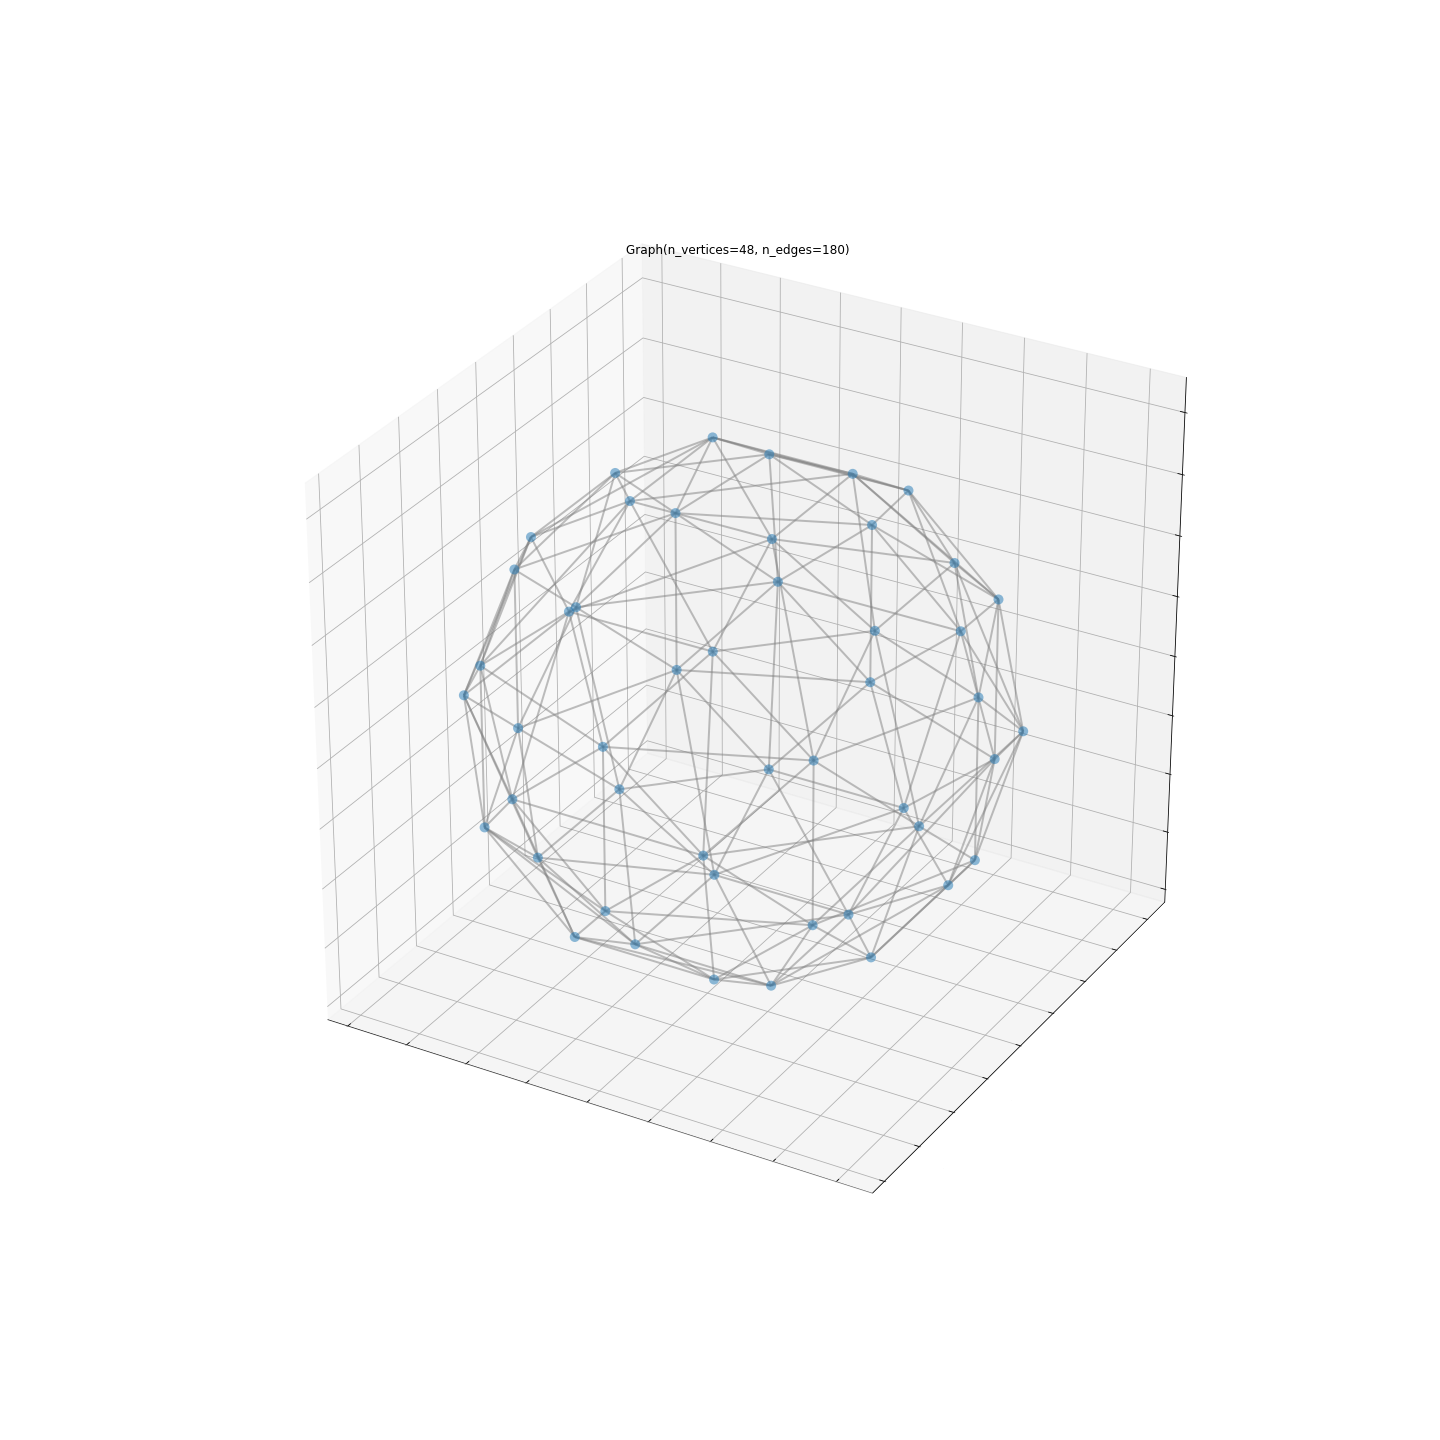
\includegraphics[width=0.8\textwidth]{figs/chapter1/graph.png}
	\caption{\label{fig:graph}Different graph topologies can drastically change the measure of smoothness of a signal $\mathbf f$, here represented as red vertical bars on the vertices.}
\end{figure}

\paragraph{Convolution and filtering on graphs}
 As the plane $\mathbb R^2$ is symmetric with respect to any translation, and the sphere $\mathbb S^2$ is symmetric with respect to any rotation, the respective definitions of convolution are equivariant respectively to these two symmetry groups. Since there are no such global symmetries in a general graph $G$, definitions (\ref{eq:plane convolution}), (\ref{eq:convolution}) can not be extended naturally on graphs. However, both on $\mathbb R^2$ and on $\mathbb S^2$, the convolution of a signal $f$ with a kernel $k$ can be performed in the spectral domain by multiplying the transformed signal $\hat f$ times the transformed kernel $\hat k$: 
\begin{equation}\label{eq:convolution normal}
f*k = \mathcal F^{-1}(\hat f \cdot \hat k)
\end{equation}
In a similar way we can define a notion of convolution also in the graph spectral domain. We use the following definition \cite{Vandergheynst} of the convolution of a signal $\mathbf f$ times a kernel $\mathbf K$:
\begin{equation}\label{eq:graph convolution}
	\Omega_\mathbf K\mathbf f = \mathcal{F}^{-1}_G(\mathbf K \hat {\mathbf f})= \mathbf V\mathbf K  \mathbf V^\intercal {\mathbf f}
\end{equation}
where $\mathbf K$ is a \textit{diagonal} \textit{matrix} $K_{ii} = k_i$. Graphs convolutions are different from the ones we are used to define in Euclidean domains, since the graph kernels $\mathbf K$ are diagonal matrices that can not be thought as the Fourier transform of a corresponding kernel defined in the spatial (vertex) domain. The diagonal elements $k_{i}$ can be thought as functions of the corresponding eigenvalues 
$$
k_{i}= k(\lambda_i)
$$
thus providing an intuitive frequency interpretation of the kernel $\mathbf K$. In this way the convolution can be seen as a \textit{filtering} operation: for example, a kernel $k(\lambda_i) = \exp (-\lambda_i)$ will be the kernel of a low-pass filter since it will cut the high frequencies.

\subsection{The Equivariance error for graph convolutions}
Take a sampling scheme $V=\{v_i\in\mathbb S^2, i=0, ..., n\}$ of the sphere, a weighted undirected graph $G(V, E, \mathbf W)$, a signal $f: \mathbb S^2\to\mathbb R$ and its sampled representation $\mathbf f:\ f_i=f(v_i)$. Suppose that there exists a sampling operator $T_V: L^2(\mathbb S^2) \supset F\to \mathbb R^n,\  T_V(f) = \mathbf f$ defined on a suitable subspace $F$ of $L^2(\mathbb S^2)$ such that it is invertible, i.e., we can unambiguously reconstruct the function $f\in F$ from its sampled values $\mathbf f$. The existence of such subspace depends on the sampling scheme $V$, and its characterization is a common problem in signal processing \cite{Driscoll:1994:CFT:184069.184073}. Recall the definition (\ref{eq:rotation operator}) of the rotation operator $\Lambda(g), g\in SO(3)$. 

We now want to understand how to set the edges and the weights of $G$ such that
\begin{equation}\label{eq:equivariance}
T \Lambda(g) T^{-1} \Omega_k T f = \Omega_k T \Lambda(g) f
\end{equation}
i.e., the graph convolution $\Omega_k$ and any rotation $\Lambda(g)$ commute.

Verifying equation (\ref{eq:equivariance}) is really hard in practice, due to the fact that for almost all samplings schemes $V$ it is not known if there exists a space $F$ in which $T$ is invertible. A special case is the \textit{equiangular sampling} scheme described in section \ref{sec:Chapter3: Heat Kernel Graph Laplacian on the Equiangular Sampling} where the sampling theorem \ref{theo:equiangular sampling theorem} holds \cite{Driscoll:1994:CFT:184069.184073}. With all the other sampling schemes, there are no sampling theorems available, but there are implementations of discrete SHT to reconstruct a sampled signal $\mathbf f$, thus providing a way to approximate $T^{-1}$. Thanks to this we are able, for a given sampling, a given function $f$, a given rotation $g$, and a given kernel $k$, to compute the \textit{normalized equivariance error} 
\begin{equation}\label{eq:equivariance error}
E_{G}(f, g) = \left(\frac{ \norm {T \Lambda(g) T^{-1} \Omega_k Tf - \Omega_k T \Lambda(g) f}_{L^2(\mathbb R^2)}}{\norm {Tf}_{L^2(\mathbb R^2)}}\right)^2
\end{equation}
where $T^{-1}$ is substituted with a discrete SHT in case $T$ is not invertible.
A measure of how equivariant a graph is with respect to rotations will then be given by the \textit{mean equivariance error}
\begin{equation}\label{eq:mean equivariance error}
\overline E_G = \mathbb E_{f, g}\ 	E_G(f, g) 
\end{equation}
In practice the expected value is obtained by averaging over a finite number of random functions and random rotations. The mean equivariance error $\overline E_G$ gives us an indication of how close the graph $G$ is from being equivariant to rotations. Now we state an intuitive concept that explains how to construct rotation invariant graphs, i.e. graphs such that $\overline{E_G}$ is small.
\begin{snugshade*}
	The mean equivariance error $\overline{E_G}$ will be small if the scalar product $\mathbf f^\intercal \mathbf v_{i(\ell, m)}$ well approximates $\hat {f}(\ell,m)$ i.e., the $L^2$ scalar product of the continuous signal \\
	$\hat {f}(\ell,m)= \int_{\eta \in \mathbb S^2}f(\eta)Y_\ell^m(\eta)d\mu(\eta)$.
	
	\textit{If $V$ is an equal area sampling scheme}, i.e. the area around each pixel $v_i$ is the same, $\overline{E_G}$ will be small if the graph Laplacian $\mathbf L$ is such that its eigenvectors $\mathbf v_i$ well approximate the eigenfunctions of the Laplace-Beltrami operator $\Delta_{\mathbb S^2}$ evaluated in the points of the sampling scheme, i.e., 
	$$
	\mathbf v_{i(\ell, m)} \approxeq Y_\ell^m(x_i)
	$$
\end{snugshade*}

In this way we framed the problem of constructing a rotation invariant graph with the more general problem of coming up with a matrix $\mathbf L$ with some specific spectral properties. Graphs are only one of many ways of coming up with such matrix $\mathbf L$, and many other methods have been already studied in the literature. In the next Chapter we present a brief overview of some of these methods providing the general context in which graph filtering can be framed.

\pagebreak

%*******************************************************************************
%*********************************** Second Chapter *****************************
%*******************************************************************************
%!TEX root = 0.main.tex
\section{First Month}
\subsection{Daniel Spielman's notes, Jupyter Notebook "Experience1" and meeting of Tuesday 26 February}

One interesting thing:

\begin{theorem}{\textit{Lemma 5.2.1 of Daniel Spielman's Lecture Notes of the course of Spectral Graph Theory (2015)}}
	\label{theo:eigenvectors on the ring}
	The Laplacian of the 2-Nearest-Neighbours ring graph $R_n$ on $n$ equispaced vertices has eigenvectors
	$$\mathbf x_k(u) = \cos(2k\pi u/n)$$
	$$\mathbf y_k(u) = \sin(2k\pi u/n)$$
	for $0\leq k\leq n/2$, ignoring $\mathbf y_0 = \mathbf 0$ and for even $n$ ignoring $\mathbf y_{n/2}$ for the same reason. Eigenvectors $\mathbf x_k, \mathbf y_k$ have eigenvalues $2-2\cos(2\pi k/n)$
\end{theorem}

This lemma make us realize the fact that for a Graph Laplacian it is possible to have eigenvectors equal to the spherical harmonics sampled in the nodes, but has completely different eigenvalues! Furthermore, if I artificially build a matrix $L'=U\Lambda'U^T$ such that $L=U\Lambda U^T$ but with $\Lambda'=\text{diag}\{-1, -4, -4, -9, -9, ...\}$ the eigenvalues of the operator  
$$\triangle \Phi(\rho, \theta) = \frac{1}{\rho}\partial_\rho \left(\frac{1}{\rho}\partial_\rho \Phi\right) + \frac{1}{\rho^2}\partial_{\theta\theta}\Phi$$ 
Laplace-Beltrami on the circle  So, this tells us that the problem proposed by Micha\"el
\begin{equation}\label{eq:michaelsproblem}
	W^\star = \arg\min_W||U-\hat U||, \quad L=D-W,\quad LU=U\Lambda
	 \hat U = \text{"Spherical harmonics sampled in the point set P"}
\end{equation}

could be badly posed, in the sens that once found the weights $W^\star$ that give us the $U^\star$ realizing the minimum above, we have no clue of which eigenvalues to set in order to retrieve a true Graph Laplacian (positive diagonal, negative entries, symmetric, row/column sum equal to $0$).\\
Nathana\"el proposes a different approach. After having observed that given a non-uniform sampling (that's the setting we are aiming at) the vectors of the spherical harmonics sampled in the point set $P$ won't be orthogonal, and thus a spectral decomposition of the Laplacian will never realize Micha\"el's problem \ref{eq:michaelsproblem} he proposes the following problem:
\begin{equation}\label{eq:nathanaelsproblem}
	\arg\min_W||L\hat U-\hat U\hat \Lambda||_\mathcal F,\quad L=D-W,\quad  W>0,\quad D=\text{diag}\{\sum_{i}(W)_{i,j}\}
\end{equation}

where $\hat{\Lambda}, \hat{U}$ are respectively the eigenvalues and eigenvectors of $\triangle_\mathcal M$ the operator of Laplace-Beltrami sampled in the point set P. In this way we get the graph laplacian that has the closest spectral decomposition to the "true" one. The problem \ref{eq:nathanaelsproblem} can be rewritten in the following form 

\begin{equation}\label{eq:nathanaelsproblem2}
[w^\star\ \lambda^\star]^T = \arg\min_W||A[w\ \lambda]^T||_2^2
\end{equation}

However, Micha\"el is not convinced by the fact that the form of the problem seems redundant: $\lambda=\lambda(w)$ is a function of $w$. So, the optimization is done on both $\lambda, w$ that can't respect the relationship $\lambda=\lambda(w)$. At the end only one of the two arguments of the minimization problem $[w^\star\ \lambda^\star]^T$ will be used to obtain the second according to the relation $\lambda=\lambda(w)$.

Waiting for Nathan\"el's notes to make this passage clearer


\subsection{Nath's problem}

Given a matrix $U$, we would like to find a valid graph such that
its eigenbase is as close to $U$ as possible. Note that $U$ might
contain only a few eigenvectors (be rectangular) and might not be
orthogonal, i.e.: $UU^{*}\neq I$.

\subsection*{Some remarks}
\begin{itemize}
	\item The Fourier basis (DFT) is probably only available for a circulant
	matrix
	\item If $U$ is not orthogonal, it is useless to try to use it directly
	to build the Laplacian
	\item The value of the eigenvalues $\Lambda$ cannot be known in advance
	\item Learning a graph given an eigenbasis has been done \cite{pasdeloup2018characterization,shafipour2017network}
	It does not work well according to me and I do not like the papers.
	\item For graph learning, the best paper to read is probably \cite{kalofolias2016learn}.
	Some more advanced results are availlable in \cite{kalofolias2018large}.
	I might be biased in recommending these two papers. You can check
	the references inside if you want to see more.
\end{itemize}

\subsection*{Problem formulation}

Solving the problem directly, i.e. searching for $U$ and $\Lambda$
is, according to me, too complicated. Hence I propose an indirect
solution. Instead of searching for $U,\Lambda$ such that $L=U\Lambda U^{*}$,
we search for $L$ such that:

\[
LU=\Lambda U
\]
We formulate the optimization problem as:

\[
\text{arg}\min_{w}\|LU-\Lambda U\|_{F}^{2}\hspace{1em}\text{s.t.}\lambda^{*}\mathbf{1}=1,w\geq0,\lambda\ge0
\]
Here $w\geq0,\lambda\geq0$ ensure that we have a valid graph and
$\lambda^{*}\mathbf{1}=1$ ensures that the trivial solution $w=0$
is not selected. Now $L$ is linearly linked to $W$ by
\[
L_{ij}=\begin{cases}
-W_{ij} & \text{if }i\ne j\\
\sum_{i}W_{ij} & \text{otherwise.}
\end{cases}
\]
Let us write this operator 
\[
\ell=O_{L}w=\text{vec}\left(\text{diag}(\text{mat}(w)\mathbf{1})-\text{mat}(w)\right)
\]
For simplicity, we assume $W_{i,i}=0$. Furthermore $LU$ is also
a linear operation. Let us write the operator $O_{U}.$ We have 
\begin{align*}
\left(LU\right)_{o,p} & =\sum_{j}L_{o,j}U_{j,p}\\
& =U_{o,p}\sum_{i}W_{io}-\sum_{j}W_{o,j}U_{j,p}
\end{align*}
Similarly, we have we define $O_{\Lambda}$ such that 
\[
O_{\Lambda}\lambda=\text{vec}(\text{diag}(\lambda)U).
\]
Eventually, we have 
\[
\|LU-\Lambda U\|_{F}^{2}=\left\Vert A\left[\begin{array}{c}
w\\
\lambda
\end{array}\right]\right\Vert _{2}^{2}
\]
where $A=\left[\begin{array}{cc}
O_{U}O_{L} & O_{\Lambda}\end{array}\right]$. The problem can be solved with a quadratic programing (QP) solver.

\subsection*{Alternative problem formulation}

The previous problem formulation penalizes mostly the spectral modes associated with high eigenvalues. In an attempt to solve this issue, we can formate the quadratic term as

\[
\|\Lambda^{-1}LU-U\|_{F}^{2}=\|\Lambda^{-1}(D-W)U-U\|_{F}^{2}.
\]
This implies that the variables $w,\lambda$ are mixed and the problem
is no longer convex. Let $T=\Lambda^{-1}(D-W)=\Lambda^{-1}D-\Lambda^{-1}W,$
then 
\[
T_{ij}=\begin{cases}
-\lambda_{i}^{-1}W_{i,j} & \text{if }i\ne j\\
\lambda_{i}^{-1}\sum_{j}W_{i,j} & \text{otherwise.}
\end{cases}
\]
Now if we were to minimize the quadratic $\|TU-U\|_{F}^{2}$, a trivial
solution would be $T=I.$ I do not think, this leads anywhere. 

\subsection*{Other ideas}

Which is the closest $U$ from $U_{G}$ such that it remains orthonormal?
\[
\text{arg}\min_{U}\|U_{G}-U\|_{F}\hspace{1em}UU^{*}=I
\]

\subsection{Weeks 2-3 (26 Feb - 12 Mar)}

\subsubsection*{Nath's problem $\mathbf{\arg \min ||LU-U\Lambda||}$}
I implemented Nathana\"el's problem in the file 04\_optimization.py on a sampled ring, in order to have the possibility to refer to theorem \ref{theo:eigenvectors on the ring} that I correctly implemented in the notebook 02\_Experience1.py. Theorem \ref{theo:eigenvectors on the ring} tells us that in some cases (uniform sampling) it is possible to have as G-eigenvectors the sampled $\mathcal{M}$-eigenvectors, but with different eigenvalues! This means (as we understood with Micha\"el on Tuesday 12 March) that if we want to engineer a graph filter $F_G(f_{(P)}) = Uh(\Lambda_G)U^Tf_{(P)}$ such that is acts on the graph-spectrum of the sampled signal $f(P)$ as the continuous $\mathcal{M}$-filter $F_\mathcal M(f)_{(x)} =  \mathcal F^{-1}\left(\sum_i h_{\mathcal M}(\lambda_{\mathcal M, i}) Y_i(\omega)\right)(x)$ acts on the $\mathcal M$-spectrum of the continuous signal $f(x)$ we need to \textit{identify the graph eigenvalues with the corresponding $\mathcal M$-eigenvalues to make sure that $h_G(\lambda_{i,G}) = h_{\mathcal M}(\lambda_{i,\mathcal M}) $}.\\
We observed that the result of the optimization for uniform sampling and for non-uniform sampling. Results are the in PDM/codes/04\_optimization/04\_figs. We see a good correspondence between $\Lambda^\star$ and the eigenvalues of the optimal Laplacian $L^\star$. However, we do not observe a good correspondence between the eigenvectors and the sampled spherical harmonics. However, it is really hard to interpret the scalar product between the vectors of the sampled spherical harmonics and the eigenvectors when the sampling is not uniform!\\
\textbf{TO DO}: to compare the graph eigenvectors with the sampled spherical harmonics we did a scalar product of the vectors. However, we need to do a proper NUDFT (Non Uniform Discrete Fourier Transform https://en.wikipedia.org/wiki/Non-uniform\_discrete\_Fourier\_transform), that is a proper discretization of the integral $\int_{\mathcal S_1} u_i(x) Y_j(x) dx$ where $u(x)$ is the continuous graph eigenvector (\textbf{QUESTION}: what does this mean?) and $Y_j$ is the $j$-th spherical harmonic. The scalar product in $\mathbb R^N$ of the sampled signals corresponds to the scalar product in $L_2(\mathcal S_1)$ and thus to a DFT only for band-limited signals and in case of uniform sampling, since the vectors of the sampled harmonics are orthonormal!
\subsubsection*{G-orthogonality and $\mathcal M$-orthogonality}
It is key to distinguish between the concepts of G-orthogonality and $\mathcal M$-orthogonality. This generated a lot of confusion in the past weeks. The question is the following: what is the SHT of a signal? The answer depends on the functional setting of the class of signals we want to work with. If we define the class of signals 

$$\mathcal F = \{f: \mathcal M \rightarrow \mathbb R: SHT(f)_i = 0\quad \forall i \geq N \}$$ 

and the sampling set $P = \{x_i \in \mathcal M\}_{i=0}^N$ we have that 

$$\forall f\in \mathcal F,  \forall x\in \mathcal M \quad \mathbf f(x)=\sum \hat f_i Y_i(x)$$

Where $\mathbf {\hat f} = \{\hat f_i\} = SHT(f)$. Thus on the sampling point set $P$ we can write

$$\forall f\in \mathcal F\quad \mathbf f_{(P)}=\sum \hat f_i Y_{i(P)} = Y_P \mathbf {\hat  f}$$


If the matrix $Y_P$ of the sampled spherical harmonics is full rank, for these signals it is true that

$$\forall f \in \mathcal F \quad SHT(f) = \mathbf{\hat f} = Y_P^{-1} f_{(P)}$$

However, for a general signal on the manifold, the $SHT(f)$ is given by the Type 2 - Non Uniform Discrete Fourier Transform (Type 2 NUDFT). From my understanding, it provides an approximation of the transform since a non-uniform sampling is capable of catching all the frequencies, but once we cut the Fourier series we do not have a Shannon Theorem (perfect reconstruction of band-limited signals).\\
The NUDFT requires to set as a parameter the maximum 

On the sphere the NASA provides us with the function \lstinline {anafast} that implements a Type2-NUDFT on the HEALPix sampling out of the box. This program performs harmonic analysis of the HEALPix maps up to a user specified maximum spherical harmonic order $l_{max}$.

\subsubsection*{The first question}
For a signal $f: \mathcal M \rightarrow \mathbb R$ define $\mathbf{\hat f}_G = U^T f(P)$ and  $\mathbf{\hat f}_\mathcal M = SHT(f)$.
The question is the following: is there a graph Fourier basis $U: U^TU=I$ such that $\mathbf{\hat f}_G = \mathbf{\hat f}_\mathcal M \forall f$?

If this is true, I have a graph such that the G-spectrum is equal to the $\mathcal M$-spectrum. However, nothing is said about the eigenspaces. \textbf{In any case, the answer to this question is NO}. 
In the setting of band limited signals $\mathcal F = \{f: \mathcal M \rightarrow \mathbb R: SHT(f)_i = 0\quad \forall i \geq N \}$  if the matrix $Y_P$ is full rank we have that $U$ has to be equal to $Y$ since $\mathbf{\hat f_G} = U^Tf(P)$ and $\mathbf{\hat f_\mathcal M} = Y_P^{-1}f(P)$. Even if we relax the request asking
 
$$(\mathbf{\hat f}_{G})_i = (\mathbf{\hat f}_{\mathcal M})_i \quad\forall i \leq n<N \quad \forall f$$

still this is impossible since from this it must follow that the first $n$ columns of $Y^{-1}_P$ are orthonormal, not true for a general sampling $P$.


\subsubsection*{The second question}
Is it possible to find a graph such that the G-eigenspaces are aligned with the $\mathcal M$-eigenspaces? \textbf{Problem: It is a badly formulated question! It doesn't mean much if we do not specify it better.} The formulation 

\[Y^TU = 
\left[ {\begin{array}{ccccc}
	B_{1\times 1} & 0 & 0 & 0 & ...\\
	0 & B_{3\times 3} & 0 & 0 & ...\\
	0 & 0 & B_{5\times 5} & 0 & ...\\
	0 & 0 & 0 & B_{7\times 7} & ...\\
	... & ... & ... & ... & ...\\
	\end{array} } \right]
\]

is not clear since we are projecting the graph eigenvectors on the sampled spherical harmonics in $\mathbb R^N$, but this corresponds to nothing!! What we want is a concept of "alignment" in the continuous domain: so, a better formulation could be the following:


\[SHT(U) = 
\left[ {\begin{array}{ccccc}
	B_{1\times 1} & 0 & 0 & 0 & ...\\
	0 & B_{3\times 3} & 0 & 0 & ...\\
	0 & 0 & B_{5\times 5} & 0 & ...\\
	0 & 0 & 0 & B_{7\times 7} & ...\\
	... & ... & ... & ... & ...\\
	\end{array} } \right]
\]

But again here we have a problem: when we write $SHT(U)$ we are imagining the eigenvectors $\mathbf u_i\in \mathbb R^N$ as traces of a continuous signal $u_i(x): \mathcal M \rightarrow \mathbb R$ and what we want is actually the $SHT(u_i(x))$. The problem is that on a uniform sampling we are limited by the Shannon theorem, that means we can reconstruct the spectrum of $u_i(x)$ only up to a certain frequency, and on a non-uniform sampling we do not know anything at all! On a non-uniform sampled signal there's no way of reconstructing the spectrum, we can only approximate it with a NUDFT. 
\paragraph{Let's now limit ourself to the usual class of band-limited signals.} We know that

$$f(x) = \sum_{i=0}^N \alpha_i Y_i(x)$$

If we suppose that the graph eigenvectors $\mathbf u_j \in \mathbb R^N$ are the trace on the vertices of a "continuous graph eigenvector" $u_j(x) \in \mathcal F$ then we know that 

$$u_j(x) = \sum_{i=0}^N \alpha^j_i Y_i(x)$$

and 

$$SHT(u_i) = Y_P^{-1}u_j(P) = Y_P^{-1}\mathbf u_j$$

so the question becomes
\begin{equation}
SHT(U) = Y_P^{-1}U = \begin{bmatrix}
		B_{1\times 1} & 0 & 0 & 0 & ...\\
		0 & B_{3\times 3} & 0 & 0 & ...\\
		0 & 0 & B_{5\times 5} & 0 & ...\\
		0 & 0 & 0 & B_{7\times 7} & ...\\
		... & ... & ... & ... & ...
		\end{bmatrix} \label{eq:SHT(U)}
\end{equation}


A procedure of proving that this is impossible by absurd could be the following: multiplying eq \ref{eq:SHT(U)} by $Y_P$ we have that

$$
U = Y_P\begin{bmatrix}
B_{1\times 1} & 0 & 0 & 0 & ...\\
0 & B_{3\times 3} & 0 & 0 & ...\\
0 & 0 & B_{5\times 5} & 0 & ...\\
0 & 0 & 0 & B_{7\times 7} & ...\\
... & ... & ... & ... & ...
\end{bmatrix}
$$
 that rewritten column by columns becomes:

 $u_0 = \alpha_1\mathbf Y_0$\\
 $u_1 = \alpha_1^1 \mathbf Y_1 + \alpha_2^1 \mathbf Y_2+ \alpha_3^1 \mathbf Y_3$\\
 $u_2 = \alpha_1^2 \mathbf Y_1 + \alpha_2^2 \mathbf Y_2+ \alpha_3^2 \mathbf Y_3$\\
 $u_3 = \alpha_1^3 \mathbf Y_1 + \alpha_2^3 \mathbf Y_2+ \alpha_3^3 \mathbf Y_3$\\
 ...\\
 
 and so on. I think that the answer to this question is again a no-no: since we must impose $UU^T=I$, this means that we have to find an orthogonal basis of each eigenspace 
 $\text{span}\{\mathbf Y_0\} = \text{span}\{\mathbf u_0\},  \text{span}\{\mathbf Y_1, \mathbf Y_2, \mathbf Y_3\} = \text{span}\{\mathbf u_1, \mathbf u_2, \mathbf u_3\}, \text{span}\{\mathbf Y_4, \mathbf Y_5, \mathbf Y_6, \mathbf Y_7, \mathbf Y_8\}=\text{span}\{\mathbf u_4, \mathbf u_5, \mathbf u_6, \mathbf u_7, \mathbf u_8\}$, etc. etc. (no problem) but the problem comes in when we must impose the $\mathbb R^N$-orthogonality between the different basis of the eigenspaces! This cannot be assured in general. \textbf{TO DO: if you're not convinced by the impossibility of this, find a counter example just with the first two eigenspaces ($|P|=4 \implies \mathbf u_i, \mathbf Y_i \in \mathbb R^4, i=0,1,2,3$)}

\pagebreak

\section{The Belkin's trinity}
\subsection{Towards a theoretical foundation of Laplacian-based manifold methods}

In this paper they present two results: a pointwise probabilistic convergence of \textbf{the extension of the graph Laplacian} $\hat L_n^t$ 

$$\forall f \in C^\infty(\mathcal M)\quad  C\frac{(4\pi t_n)^{-\frac{k+2}{2}}}{n} L_n^t f(\bf x) \xrightarrow{n\to\infty}\triangle_\mathcal M f(\bf x)$$

and a uniform (pointwise convergence of the operator) one

$$\sup_{x\in\mathcal M, f\in \mathcal F_C}\left| C\frac{(4\pi t_n)^{-\frac{k+2}{2}}}{n} L_n^t f(\bf x) - \triangle_\mathcal M f(\bf x) \right|\xrightarrow{n\to\infty}0
, \quad \mathcal F_C = \left\{f\in C^\infty(\mathcal M), f^{(i)}(x)\leq M, i=1,2,3\right\}$$

here nothing is said about convergence of the spectra, plus there's nothing written about the relationship between $\mathbf{Eig} L_n^t$ (the eigenfunctions and eigenvalues of the extension of the graph Laplacian) and $\mathbf {Eig} \mathbf {L}_n^t$ (the eigenvectors and eigenvalues of the matrix Laplacian).

Theorem 1 is proven by simple analysis arguments and by Hoeffding's formula (probability). 
First, by the simple law of large numbers, we have that for a fixed $t>0$, a fixed function $f$ and a fixed point $p\in\mathcal M$
\begin{equation}\label{eq:pointwise convergence of laplacian discrete approximation}
\lim_{n\to\infty}\frac{1}{t}\frac{1}{ (4\pi t)^{\frac{k}{2}}}L_n^tf(p)= L^tf(p)
\end{equation}



where 

$$L^tf(p)=  \frac{1}{t}\frac{1}{ (4\pi t)^{\frac{k}{2}}} \int_\mathcal Me^{-\frac{||p-x||^2}{4t}}\left(f(x)-f(p)\right)d\mu(x)$$

To prove the convergence of $L^t$ to $\triangle_\mathcal M$, then we need three steps, that we can recycle completely. They use the fact that thanks to the exponential map the heat kernel centered on $p$ on any manifold can be approximated by a Gaussian in the ambient Euclidean space in a small neighborhood of $p$, and the relationship between Euclidean distances and geodesic distances.

\textbf{In order to adapt this proof to our needs, we just need to find an alternative to the law of large numbers (LLN) used to prove \ref{eq:pointwise convergence of laplacian discrete approximation}}

Theorem 2 is proven with arguments of Functional Analysis: Ascoli-Arzelà, compact convergence in Sobolev spaces, etc.etc...

\subsection{Consistency of Spectral Clustering}
 $$ \mathbf{Eig} \mathbf{L}^t_n \xrightarrow[a.s.]{n\to\infty} \mathbf{Eig} L^t $$
It aims at proving the convergence of eigenvalues and eigenvectors of random graph Laplacian matrices for growing sample size. They present two results: one for the normalized Laplacian and one for the unnormalized Laplacian. Since the matrix eigenvectors grow in dimension as the sample size increases, standard convergence arguments can not be applied. However, they show that there exists a function $f\in C(\mathcal M)$ such that the difference between the eigenvector $v_n$ and the restriction of $f$ to the sample converges to $0$

$$||v_n-\rho_nf||\rightarrow 0$$

To do so they see the eigenvector $v_n$ as the restriction to the sample of a continuous eigenfunction $f_n$ of some continuous operator $U'_n$ that acts on the space $C(\mathcal M)$. Then they use the fact that 

$$||v_n-\rho_nf||_\infty = ||\rho_nf_n-\rho_nf||_\infty\leq ||f_n-f||_\infty$$


So, it will just be necessary to show that  $$||f_n-f||_\infty\rightarrow 0$$
 \textbf{compact convergence} of both matrices towards $L^t$ (where $\mathcal M$ is a compact metric space) in the Banach space of the continuous functions $(C, ||\cdot||_\infty)$. 

Compact convergence ensures convergence of spectral properties in the following sense: for isolated eigenvalues of the limit operator $\triangle_\mathcal M$ with finite multiplicity we have convergence of eigenvalues and eigenspaces but not convergence of eigenfunctions. for isolated simple eigenvalues of the limit operator we have also convergence of the eigenfunctions!

The proof consists in three steps:
\paragraph{Step 1} Construct a bounded operator $U'_n$ on the Banach space $(C(\mathcal M), ||\cdot||_\infty)$ such that restricted on the sampled values behaves like $\mathbf{L}'_n$. Then, construct an operator $U'$ such that for the law of large numbers for a fixed $f$ and for a fixed $x$, $U'_nf(x) \xrightarrow U'f(x) $
\paragraph{Step 2} Here they establishes the connection between the spectra of $L'_n$ and $U'_n$. In particular, they prove a one-to-one correspondence between the eigenfunctions and eigenvalues of $U'_n$ and the eigenvectors and eigenvalues of $L'_n$, provided that satisfy $\lambda\notin \{1\}=\sigma_{ess}(U'_n)= \sigma_{ess}(U')$.
\paragraph{Step 3} Here we prove compact convergence:

$$U'_n \xrightarrow[n\to\infty]{c,\ a.s.}U'$$

At the light of compact convergence and on the analysis of the essential spectrum of $U'_n, U'$ and the one-to-one correspondence of the spectra done in step 2, given Proposition 6 \textit{Perturbation results for compact convergence} we get to the following result

\begin{theorem}
	Let $\lambda\neq 1 $ be an eigenvalue of $U'$ and $M\subset \mathbb C$ an open neighborhood of $\lambda$ such that $\sigma(U')\cap M=\{\lambda\}$. Then:
\begin{enumerate}
	\item Convergence of eigenvalues: The eigenvalues in$\sigma(L'_n)\cap M$ converge to $\lambda$ in the sense that every sequence $(\lambda_n)_{n\in\mathbb N}$ with $\lambda_n\in\sigma(L'_n)\cap M$ satisfies $\lambda_n\rightarrow \lambda$ almost surely.
	\item Convergence of spectral projections: There exists some $N\in\mathbb N$ such that for $n>N$, the sets $\sigma(U'_n)\cap M$ are isolated in $\sigma(U'_n)$. For $n>N$, let $Pr'_n$ be the spectral projection of $U'_n$ corresponding to $\sigma(U'_n)\cap M$, and $Pr$ the spectral projection of $U$ for $\lambda$. Then $Pr'_n\xrightarrow p Pr a.s.$
	\item Convergence of eigenvectors: if $\lambda$ is a single eigenvalue, then the eigenvectors of $L'_n$ converge a.s. up to a change of sign: if $v_n$ is the eigenvector
	of $L'_n$ with eigenvalue $\lambda_n$, $v_{n,i}$ its i-th coordinate, and $f$ the eigenfunction of eigenvalue $\lambda$, then there exists a sequence $(a_n)_{n\in\mathbb N}$ with $a_i \in \{+1,-1\}$ such that $\sup_{i=1,...,n} |a_nv_{n,i} - f(X_i)| \rightarrow 0$ a.s. In particular, for all $b \in\mathbb R$, the sets $\{a_nf_n > b\}$ and $\{f > b\}$ converge, that is, their symmetric difference satisfies $P(\{f > b\}\triangle\{a_nf_n > b\}) \rightarrow 0$.
\end{enumerate}
\end{theorem}

A similar theorem is stated also for non-normalized Laplacian matrix, although the arguments stay the same.
\subsection{Convergence of Laplacian Eigenmaps}
Here all the pieces are put together. 

 $$ \mathbf{Eig} \mathbf{ L}^t_n \xrightarrow[a.s.]{n\to\infty} \mathbf{Eig} L^t \xrightarrow{t\to0} \mathbf{Eig} \triangle_\mathcal M $$
 
 \begin{theorem}
 	Let $\lambda_{n,i}^t$ be the ith eigenvalue of $\hat L_n^t$ and $e^t_{n,i}$ be the corresponding eigenfunction (which for each fixed i will be shown to exist for t sufficiently small). Let $\lambda_{i}$ be the ith eigenvalue of $\triangle_\mathcal M$ and $e_{i}$ be the corresponding eigenfunction. Then there exists a sequence $t_n\rightarrow 0$ such that
 	
 	$$\lim_{n\rightarrow\infty} \lambda_{n,i}^{t_n}=\lambda_i$$
 	$$\lim_{n\rightarrow\infty}||e_{n,i}^{t_n}(x) - e_i(x)||_2 = 0$$
 	
 	where the limits are in probability.
 	
 \end{theorem}

\paragraph{Step 1: Spectral convergence of the empirical approximation $\mathbf{ L}_n^t$ to $L^t$}
Recycle the work of \textbf{Consistency of Spectral Clustering} with the analysis of the essential spectrum of the limit operator $\sigma_{ess}(L^t)$.
\paragraph{Step 2: Spectral convergence of the functional approximation $L^t$ to $\triangle$}
Really hard. Uniform operator convergence does not hold, however spectral convergence is still assured in theorem 4.1 of the paper. This part, although really hard, will stay the same!


\section{Pointwise convergence in the HEALPix case}

Getting inspired from the work flow presented above, we try to replicate the first theorem obtained in \textbf{Towards a theoretical foundation of Laplacian-based manifold methods} but not in the case of random Laplacians, but in the case of deterministic ones where the sampling is given by the HEALPix scheme. This analysis will be a preparatory work to further studies, since as we pointed out so far, form this kind of convergence nothing is said about the convergence of eigenvalues and eigenvectors. However, this study could maybe tell us something about the equivariance of the graph with respect to the action of the rotation group $SO(3)$.


We remind that \textbf{in order to adapt this proof to our needs, we just need to find an alternative to the law of large numbers (LLN) used to prove eq. (\ref{eq:pointwise convergence of laplacian discrete approximation}}). We know by construction that the HEALPix sampling cut the sphere into equal areas. Let us note the surface of one level $S_{N_{side}}$, and the maximum distance to the center point of one surface\textbf{ $d_{N_{side}}$}.
Let us assume that the function $f$ is $L$ Lipschitz, we have
\[
\int_{\sigma_{i}}f({\bf x})\text{d}{\bf x}-\frac{1}{2}Ld_{N_{side}}S_{N_{side}}\leq S_{N_{side}}f({\bf x}_{i})\leq\int_{\sigma_{i}}f({\bf x})\text{d}{\bf x}+\frac{1}{2}Ld_{N_{side}}S_{N_{side}}.
\]
Hence we have:
\[
\sum_{i}\int_{\sigma_{i}}f({\bf x})\text{d}{\bf x}-\sum_{i}\frac{1}{2}Ld_{N_{side}}S_{N_{side}}\leq S_{N_{side}}\sum_{i}f({\bf x}_{i})\leq\sum_{i}\int_{\sigma_{i}}f({\bf x})\text{d}{\bf x}+\sum_{i}\frac{1}{2}Ld_{N_{side}}S_{N_{side}}
\]
and 
\[
\left|S_{N_{side}}\sum_{i}f({\bf x}_{i})-\int f({\bf x})\text{d}{\bf x}\right|\le\frac{1}{2}Ld_{N_{side}}S_{tot}
\]
where $S_{tot}$ is the the total surface of the sphere. Now we need to characterize $d_{N_{side}}$ with respect of $N_{side}$ and $L$ with respect of $m$ and $\ell$. 

Now, we found the following code, part of Healpix\_cxx 2.15a \cite{Healpix_cc} that illustrates how to calculate the maximum distance between a pixel and the corner of the corresponding patch. The class \lstinline|vec3| implements a 3D cartesian vector, the function \lstinline|vec3.set_z_phi(double, double)| creates a unit vector from a z coordinate and an azimuthal angle. Both \lstinline|va| and \lstinline|vb| converge towards the point $(2/3, 0)$, making $$d_{N_{side}}\rightarrow0$$
\begin{lstlisting}[language=c++]
	double Healpix_Base::max_pixrad() const
	{
		vec3 va,vb;
		va.set_z_phi (2./3., pi/(4*nside_));
		double t1 = 1.-1./nside_;
		t1*=t1;
		vb.set_z_phi (1-t1/3, 0);
		return v_angle(va,vb);
	}
\end{lstlisting}

\pagebreak

\iffalse
\clearpage
\appendix
\fi

\bibliography{references.bib} 

\nocite{*}

\pagebreak



\end{document}
